\subsection{Metodologia Espectral e Resultados Numéricos}

A resolução do problema $ (\nabla^2 + I)F = 3e^{x+y} $ em malhas de Chebyshev foi modularizada no pacote \texttt{SpectralTools} e consumida pelo projeto \texttt{\_hw\_10}. O pipeline é definido em \texttt{solve\_anisotropic.jl}, onde a função genérica \texttt{solve\_rectangular\_case} constrói os operadores 1D/2D, impõe contornos e reconstrói o campo:

\begin{lstlisting}[language=Julia]
x  = cheb_lobatto_nodes(nx)
y  = cheb_lobatto_nodes(ny)
_, D2x = cheb_D_matrices(nx)
_, D2y = cheb_D_matrices(ny)
X, Y = grid2D(x, y)

A    = laplacian_plus_I_operator(D2x, D2y)
rhs  = 3 .* exp.(X .+ Y)
mask = build_internal_mask(size(X))

Ared, bred, _ = apply_dirichlet!(A, vec(rhs), mask, exp.(X .+ Y))
F_internal    = solve_poisson_like(Ared, bred)
solution      = rebuild_solution(F_internal, exp.(X .+ Y), mask)
\end{lstlisting}

O ponto crítico para garantir consistência entre malhas isotrópicas e anisotrópicas está no gerador de operadores 2D. Inicialmente, o caso anisotrópico apresentava uma solução incorreta devido a uma inversão na ordem dos produtos de Kronecker: o termo $kron(I_y, D^{(2)}_x)$ foi trocado por $kron(D^{(2)}_x, I_y)$ (e análogo para $y$), fazendo com que as derivadas atuassem em direções trocadas quando $n_x \neq n_y$. O trecho abaixo mostra a implementação corrigida (\texttt{SpectralTools/src/Operators2D.jl}):

\begin{lstlisting}[language=Julia]
function laplacian_plus_I_operator(D2x::AbstractMatrix, D2y::AbstractMatrix)
    nx, ny = size(D2x, 1), size(D2y, 1)
    Ix = Matrix{Float64}(I, nx, nx)
    Iy = Matrix{Float64}(I, ny, ny)

    A = kron(Ix, D2y) + kron(D2x, Iy) + I(nx * ny)
    return sparse(A)
end
\end{lstlisting}

Após essa correção, os resultados dos casos anisotrópico $(15 \times 20)$ e isotrópicos $(15 \times 15)$ e $(20 \times 20)$ convergiram para o mesmo perfil analítico, com diferenças apenas na magnitude do erro numérico.

\paragraph{Figuras.} As Figuras~\ref{fig:solution-aniso}--\ref{fig:heatmap-iso20} exibem as soluções e erros para todos os cenários:
\begin{itemize}
    \item \textbf{Figuras~\ref{fig:solution-aniso}, \ref{fig:solution-iso15}, \ref{fig:solution-iso20}} comparam as superfícies numéricas dos três casos, evidenciando que todos reproduzem $e^{x+y}$ visualmente.
    \item \textbf{Figuras~\ref{fig:error-surface-aniso}, \ref{fig:error-surface-iso15}, \ref{fig:error-surface-iso20}} mostram os resíduos nas malhas de Chebyshev; percebe-se que a malha anisotrópica e a isotrópica de ordem 20 apresentam erros de mesma ordem, enquanto a isotrópica de ordem 15 sofre leve degradação.
    \item \textbf{Figuras~\ref{fig:heatmap-aniso}, \ref{fig:heatmap-iso15}, \ref{fig:heatmap-iso20}} trazem mapas de calor após interpolação uniforme $101\times101$, corroborando a estabilidade da solução em todo o domínio.
\end{itemize}

\begin{figure}[htbp]
    \centering
    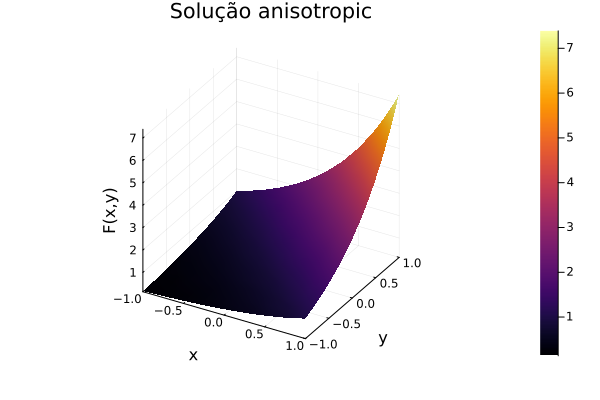
\includegraphics[width=0.32\textwidth]{figures/solution_anisotropic.png}
    \caption{Solução numérica $F(x,y)$ para o caso anisotrópico $(15,20)$.}
    \label{fig:solution-aniso}
\end{figure}

\begin{figure}[htbp]
    \centering
    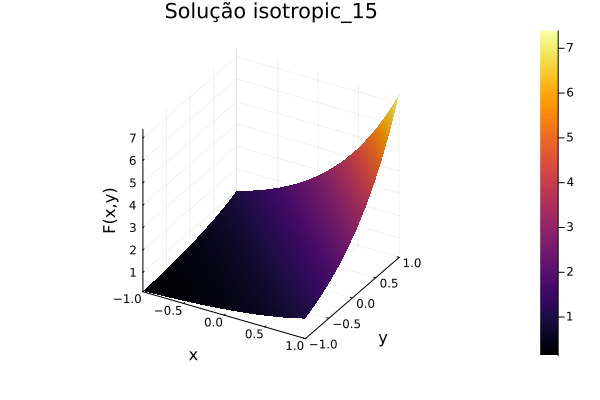
\includegraphics[width=0.32\textwidth]{figures/solution_isotropic_15.png}
    \caption{Solução isotrópica com $N_x=N_y=15$.}
    \label{fig:solution-iso15}
\end{figure}

\begin{figure}[htbp]
    \centering
    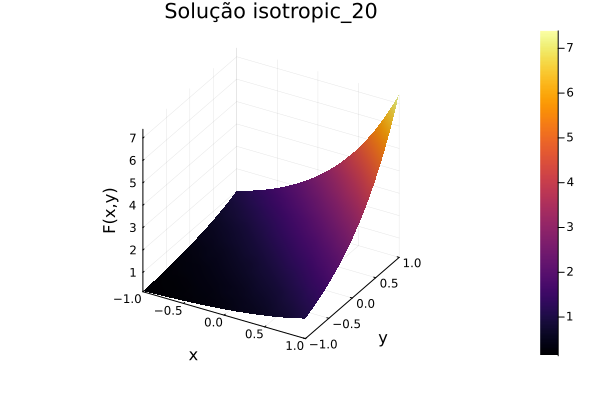
\includegraphics[width=0.32\textwidth]{figures/solution_isotropic_20.png}
    \caption{Solução isotrópica com $N_x=N_y=20$.}
    \label{fig:solution-iso20}
\end{figure}

\begin{figure}[htbp]
    \centering
    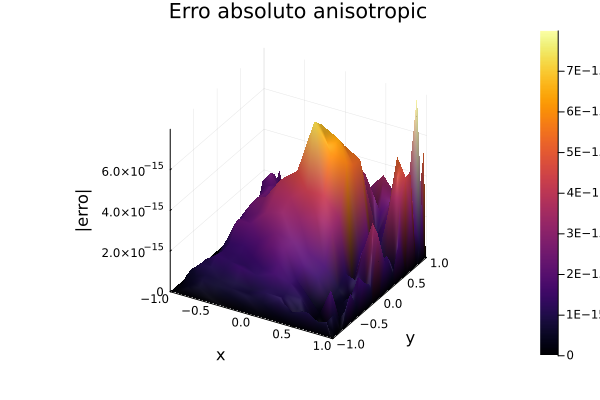
\includegraphics[width=0.32\textwidth]{figures/error_surface_anisotropic.png}
    \caption{Erro absoluto na malha de Chebyshev (anisotrópico).}
    \label{fig:error-surface-aniso}
\end{figure}

\begin{figure}[htbp]
    \centering
    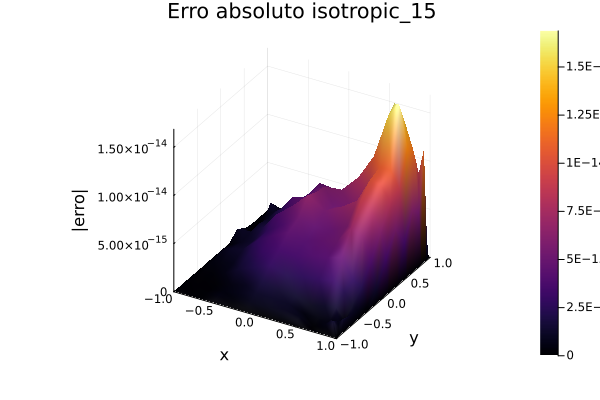
\includegraphics[width=0.32\textwidth]{figures/error_surface_isotropic_15.png}
    \caption{Erro absoluto na malha de Chebyshev (isotrópico 15).}
    \label{fig:error-surface-iso15}
\end{figure}

\begin{figure}[htbp]
    \centering
    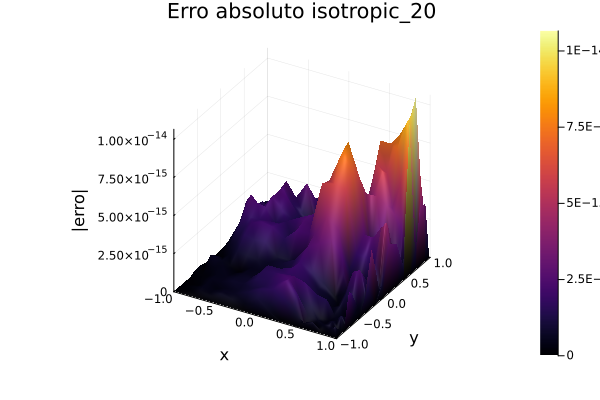
\includegraphics[width=0.32\textwidth]{figures/error_surface_isotropic_20.png}
    \caption{Erro absoluto na malha de Chebyshev (isotrópico 20).}
    \label{fig:error-surface-iso20}
\end{figure}

\begin{figure}[htbp]
    \centering
    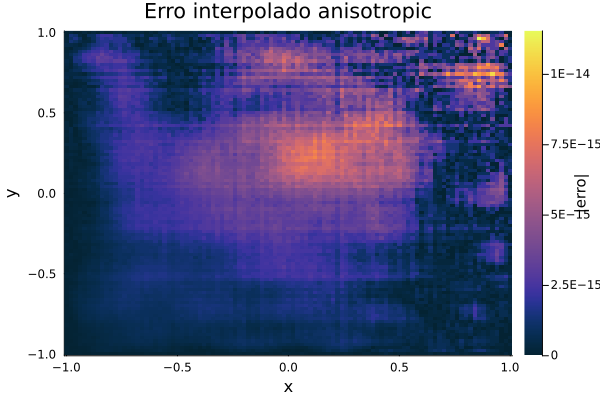
\includegraphics[width=0.32\textwidth]{figures/error_heatmap_anisotropic.png}
    \caption{Erro interpolado em grade uniforme (anisotrópico).}
    \label{fig:heatmap-aniso}
\end{figure}

\begin{figure}[htbp]
    \centering
    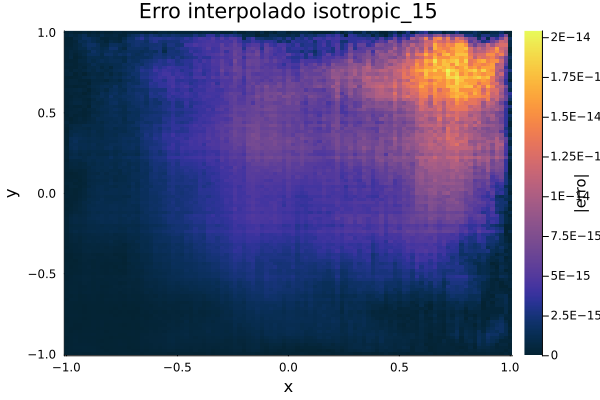
\includegraphics[width=0.32\textwidth]{figures/error_heatmap_isotropic_15.png}
    \caption{Erro interpolado em grade uniforme (isotrópico 15).}
    \label{fig:heatmap-iso15}
\end{figure}

\begin{figure}[htbp]
    \centering
    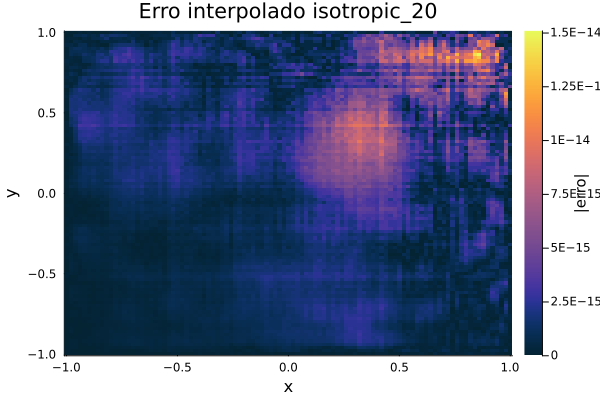
\includegraphics[width=0.32\textwidth]{figures/error_heatmap_isotropic_20.png}
    \caption{Erro interpolado em grade uniforme (isotrópico 20).}
    \label{fig:heatmap-iso20}
\end{figure}

\paragraph{Tabelas de erro.} As métricas consolidadas em \texttt{data/summary.txt} são resumidas na Tabela~\ref{tab:errors}. Todas as abordagens atingem erros máximos na ordem de $10^{-14}$, mas apresentam nuances:

\begin{table}[htbp]
    \centering
    \begin{tabular}{lcccc}
        \toprule
        Caso & $\|e\|_{\infty}$ (Cheb.) & $\|e\|_{2}$ (Cheb.) & $\|e\|_{\infty}$ (Uni.) & $\|e\|_{2}$ (Uni.) \\
        \midrule
        Anisotrópico $(15,20)$ & $7.99\times10^{-15}$ & $1.97\times10^{-15}$ & $\mathbf{1.15\times10^{-14}}$ & $2.67\times10^{-15}$ \\
        Isotrópico $(15,15)$   & $1.69\times10^{-14}$ & $4.13\times10^{-15}$ & $2.04\times10^{-14}$ & $5.09\times10^{-15}$ \\
        Isotrópico $(20,20)$   & $1.07\times10^{-14}$ & $\mathbf{2.24\times10^{-15}}$ & $1.51\times10^{-14}$ & $\mathbf{2.60\times10^{-15}}$ \\
        \bottomrule
    \end{tabular}
    \caption{Erros máximos e L2 nas malhas de Chebyshev e uniforme (\texttt{data/summary.txt}).}
    \label{tab:errors}
\end{table}

O caso anisotrópico destaca-se pelo menor erro máximo tanto na malha original quanto na interpolada, pois distribui mais pontos na direção $y$, acompanhando melhor a curvatura da solução ao longo dessa direção. Já o caso isotrópico com $20$ pontos por direção apresenta os menores erros L2 (tanto na malha espectral quanto na uniforme), refletindo a maior resolução total. Portanto, se o critério é minimizar o erro máximo com o menor custo computacional, o caso anisotrópico $(15,20)$ é preferível; se o foco é reduzir o erro global em norma L2 e há orçamento para um grid maior, o isotrópico $(20,20)$ leva vantagem.

Em suma, após corrigir a montagem do operador via produtos de Kronecker, ambos os estilos de malha convergiram para a mesma solução analítica, e a escolha entre anisotrópico ou isotrópico passa a ser orientada apenas pelos requisitos de precisão versus custo computacional.
